\documentclass[12pt, a4paper]{article}
\usepackage[margin = 1in, top=1.3in]{geometry}
\usepackage[english]{babel}
\usepackage[utf8]{inputenc}
\usepackage{fancyhdr}
\usepackage{amsmath}
\usepackage{bm}
\usepackage{graphicx}
\usepackage{subcaption}
\usepackage[font=small,labelfont=bf]{caption}
 
\pagestyle{fancy}
\fancyhf{}
\rhead{\small{Shaan Ul Haque(180070053)\\ Samarth Singh (180050090) \\ Niraj Mahajan (180050069)}}
\lhead{CS-663 Assignment-1 : Question 1}
\rfoot{Page 1.\thepage}
 
\begin{document}
\vspace*{-22pt}
\section*{Question 1}
\subsection*{Part A}
Moire Patterns occur when we undersample an image. Below you can find the striking difference between original image and the undersampled images. Here undersampling factor is denoted by d.

\begin{figure}[h!]
  \centering
    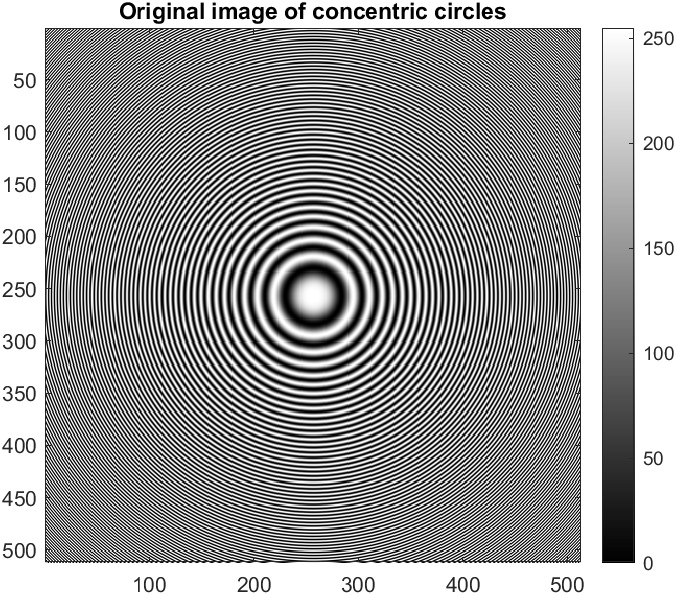
\includegraphics[scale=0.8]{ConcentricCircles_original.png}
    \caption{Concentric Circles}
  \label{fig:1}
\end{figure}

\begin{figure}[h!]
  \centering
    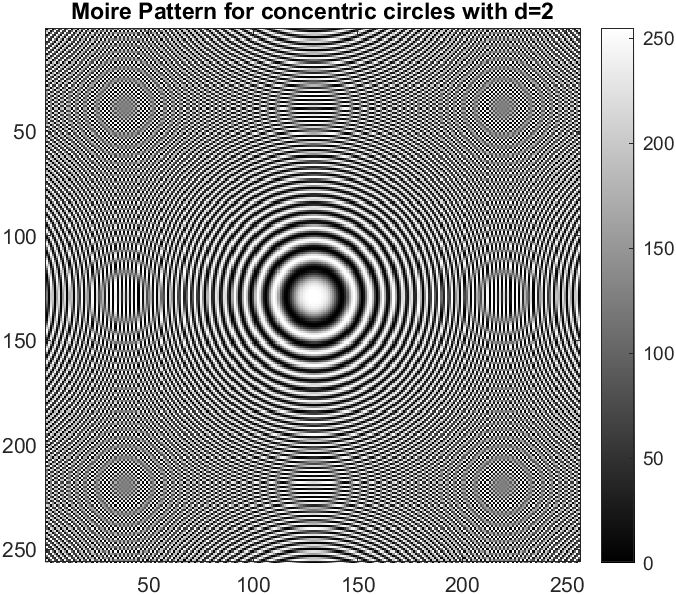
\includegraphics[scale=0.8]{moire2.png}
    \caption{}
  \label{fig:1}
\end{figure}

\begin{figure}[h!]
  \centering
    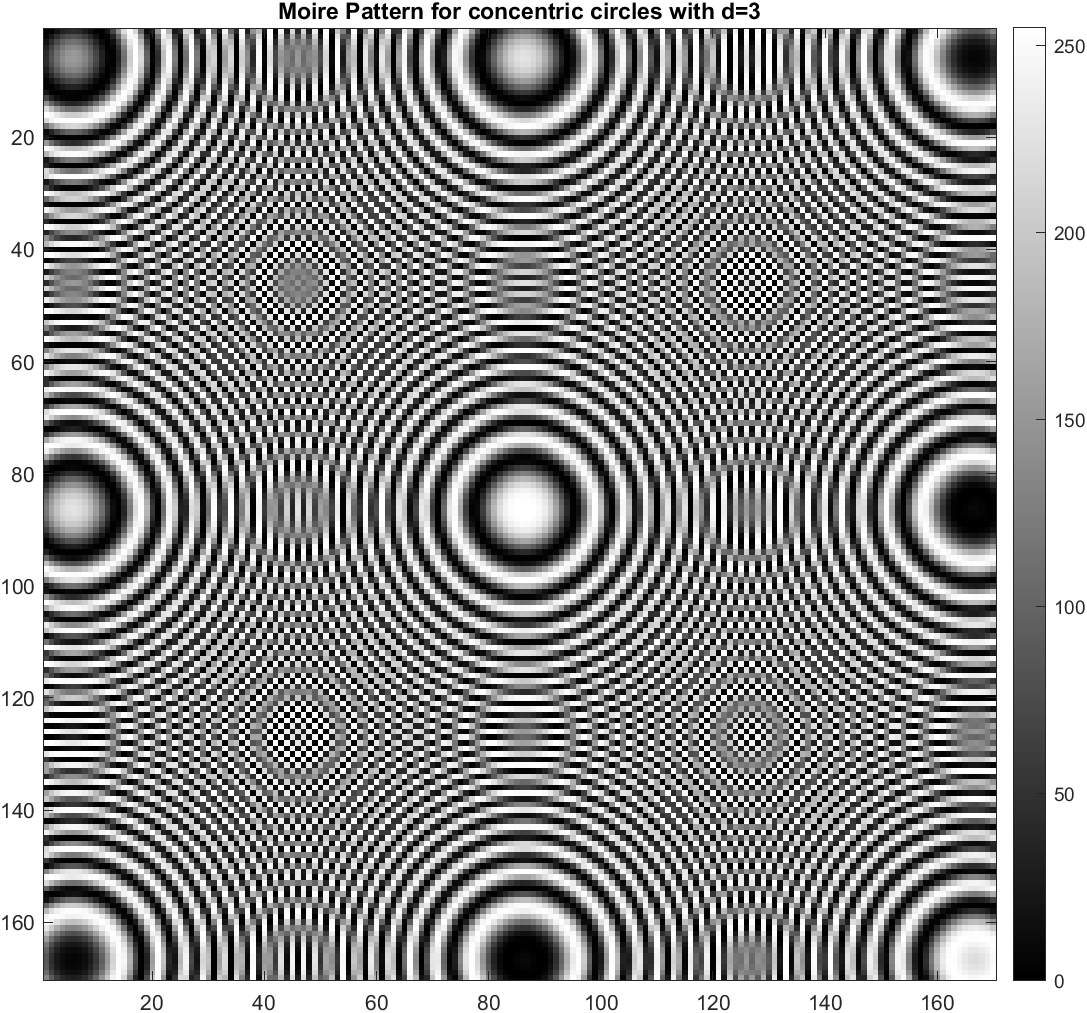
\includegraphics[scale=0.5]{moire3.png}
    \caption{}
  \label{fig:1}
\end{figure}

\subsection*{Part B}
Here the original image is an N*N pixel dimensional image, where N=103. We want to enlarge the image by increasing the image pixel dimensions. The increment is as follows:

\begin{equation*}
    new\_rows=3*M-2,\ where\ M=number\ of\ rows\\
\end{equation*}

\begin{equation*}
    new\_cols=2*M-1,\ where\ N=number\ of\ columns\\
\end{equation*}

Here M=N.\\
We used different interpolation techniques. This part is for Bilinear Interpolation. Results are shown in next page:

\begin{figure}[h!]
  \centering
    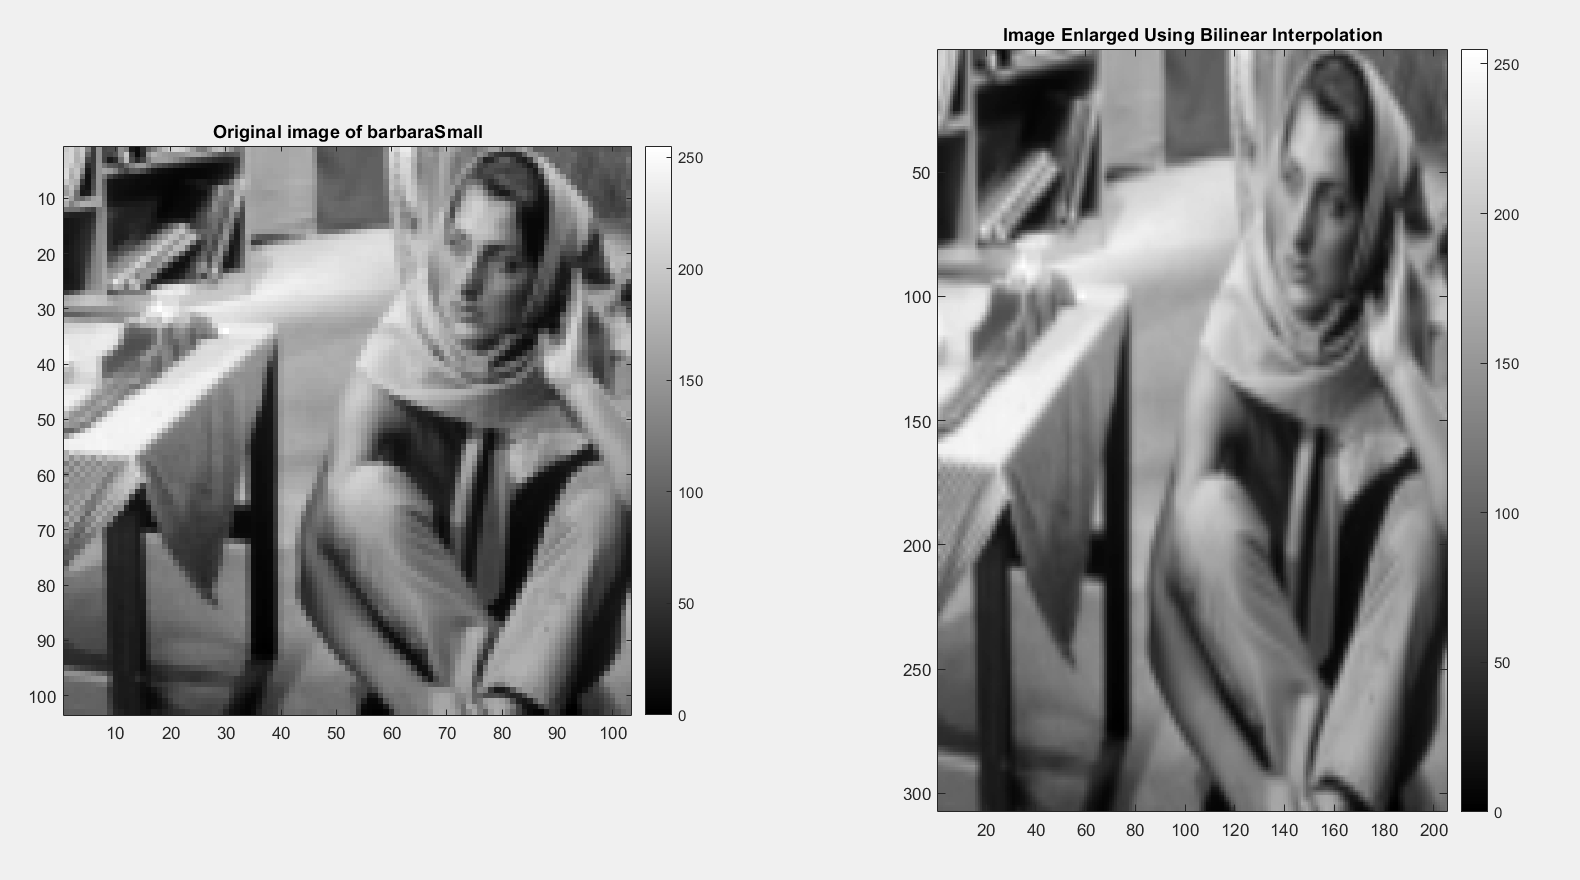
\includegraphics[scale=0.4]{bilinear.png}
    \caption{Bilinear Interpolation}
  \label{fig:3}
\end{figure}

\subsection*{Part C}
This part has has the same requirements as needed previously only we interpolated the function using nearest neighbor.Results are shown in next page:

\begin{figure}[h!]
  \centering
    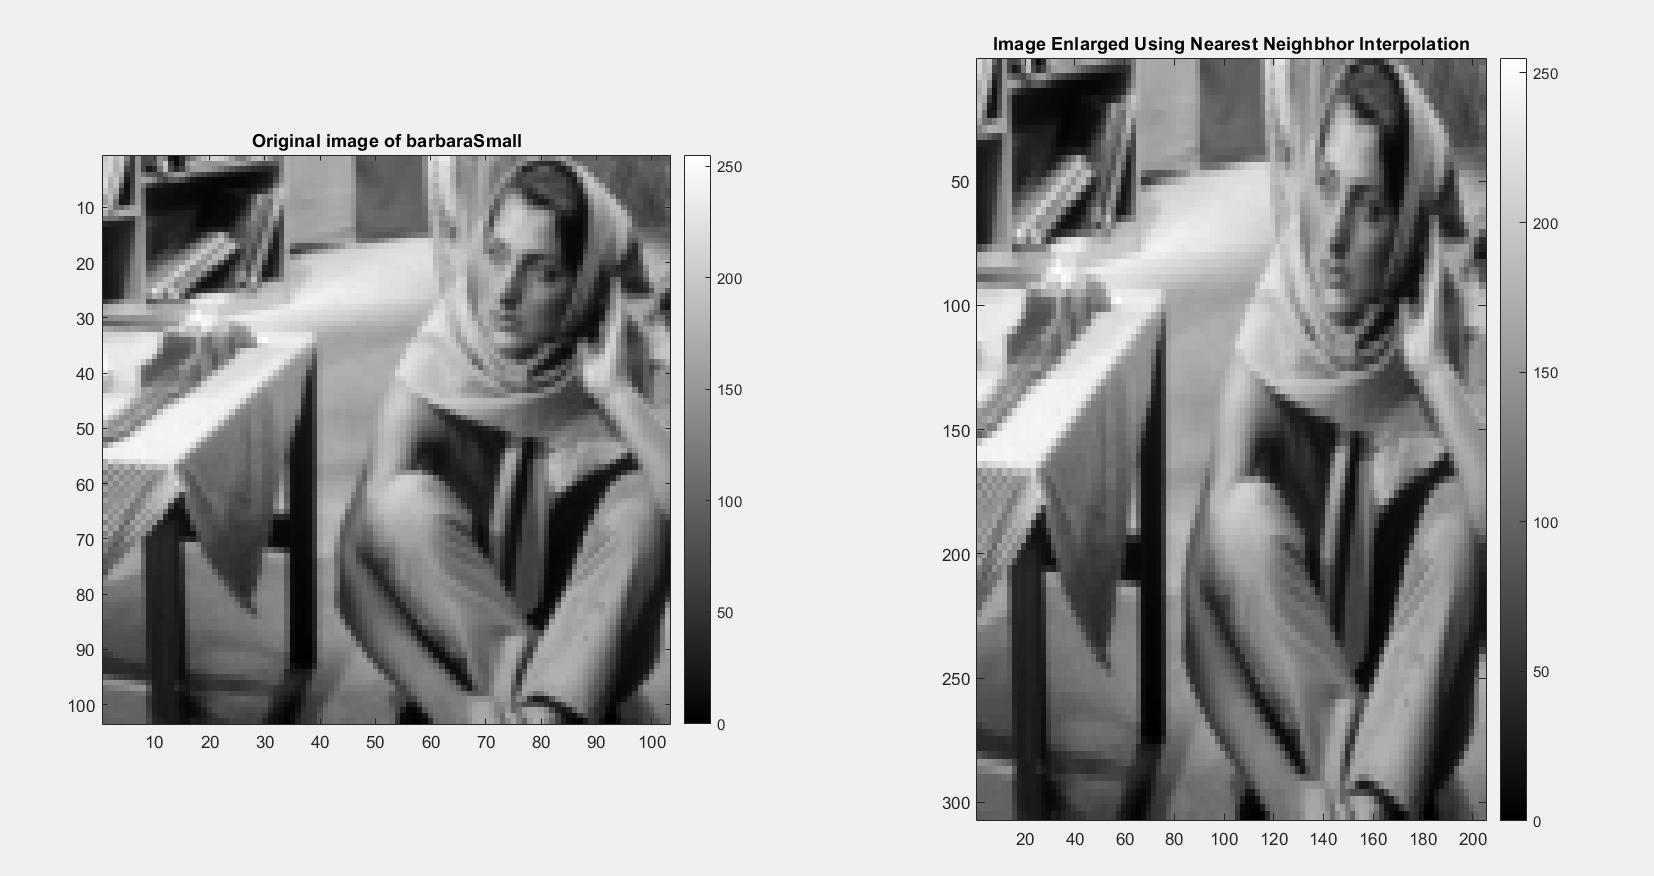
\includegraphics[scale=0.4]{nearest_neighbor.png}
    \caption{Nearest Neighbor Interpolation}
  \label{fig:4}
\end{figure}

\clearpage

\subsection*{Part D}
Again, this part also has has the same requirements as needed previously only we interpolated the function using bicubic interpolation.Results are shown below:

\begin{figure}[h!]
  \centering
    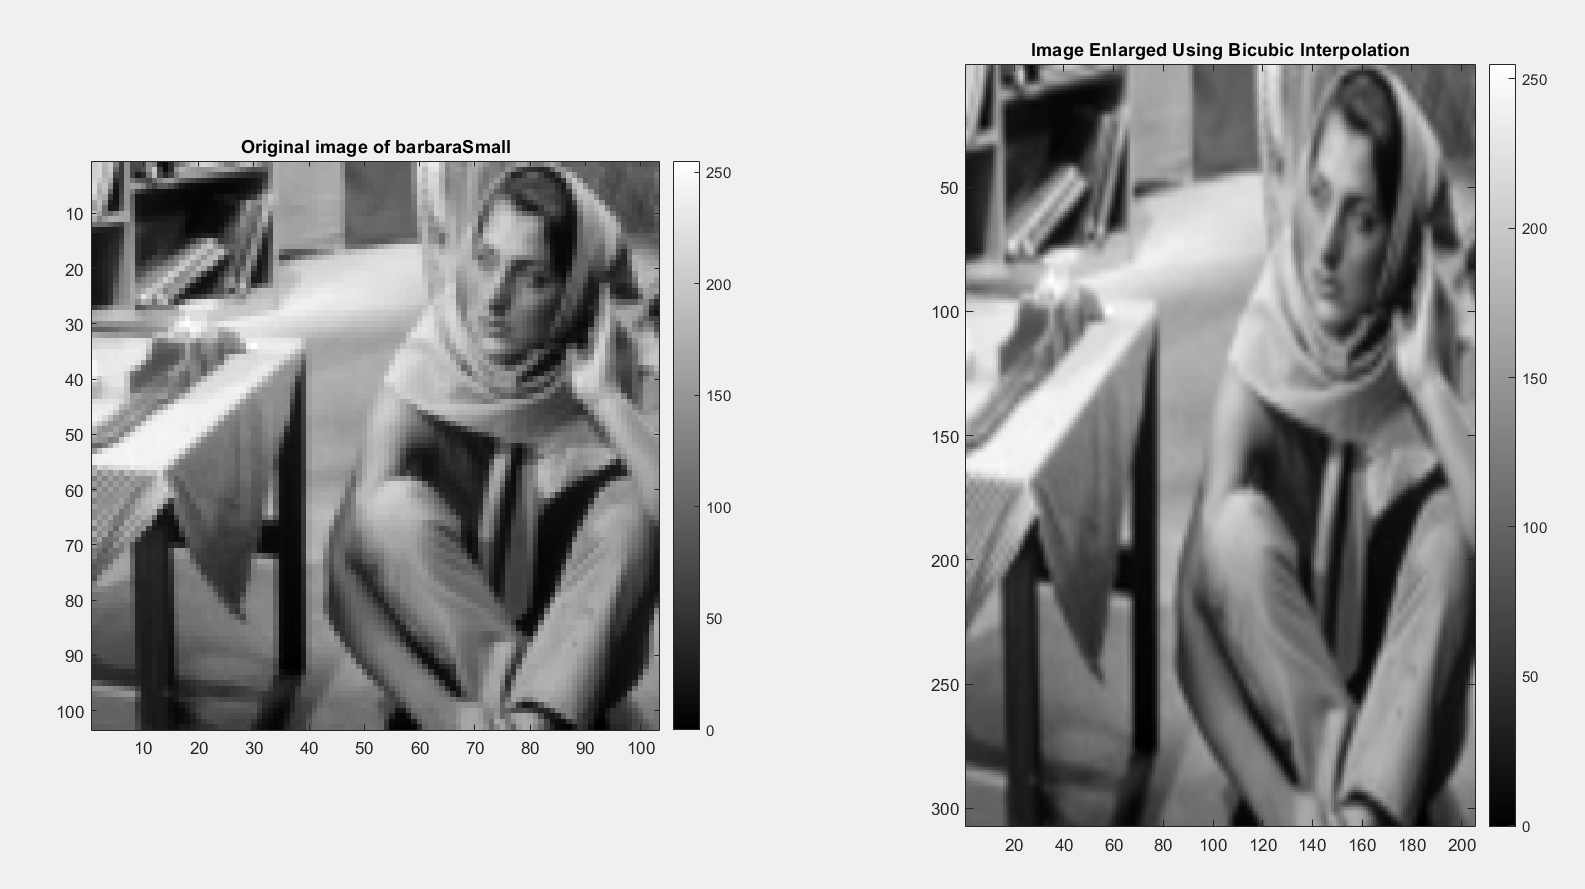
\includegraphics[scale=0.4]{bicubic.png}
    \caption{Bicubic Interpolation}
  \label{fig:5}
\end{figure}

\subsection*{Part E}
The coarsest image obtained was from nearest neighbor interpolation. This interpolation method just looks at the nearest function value from a required point and assigns it the same value thus leads to very pixelated image.\\
Bilinear interpolation approximates the function using linear approximation thus leads to better image. Though the function value is continuous everywhere the derivative is discontinuous at given function points.\\
Bicubic interpolation approximates the function using cubic approximation thus leads to even better image. The interpolated function generated is continuous as well as its first derivative is also continuos a every point. The image is smoothest generated by this method. \\

We took a small patch of image and used colormap to generate the differences. Though bilinear and bicubic give almost same results but we find smoother transition from darker to lighter pixel intensities in bicubic technique (especially in red and blue regions). in the image are  Results are shown in next page. 
\begin{figure}[h!]
  \centering
    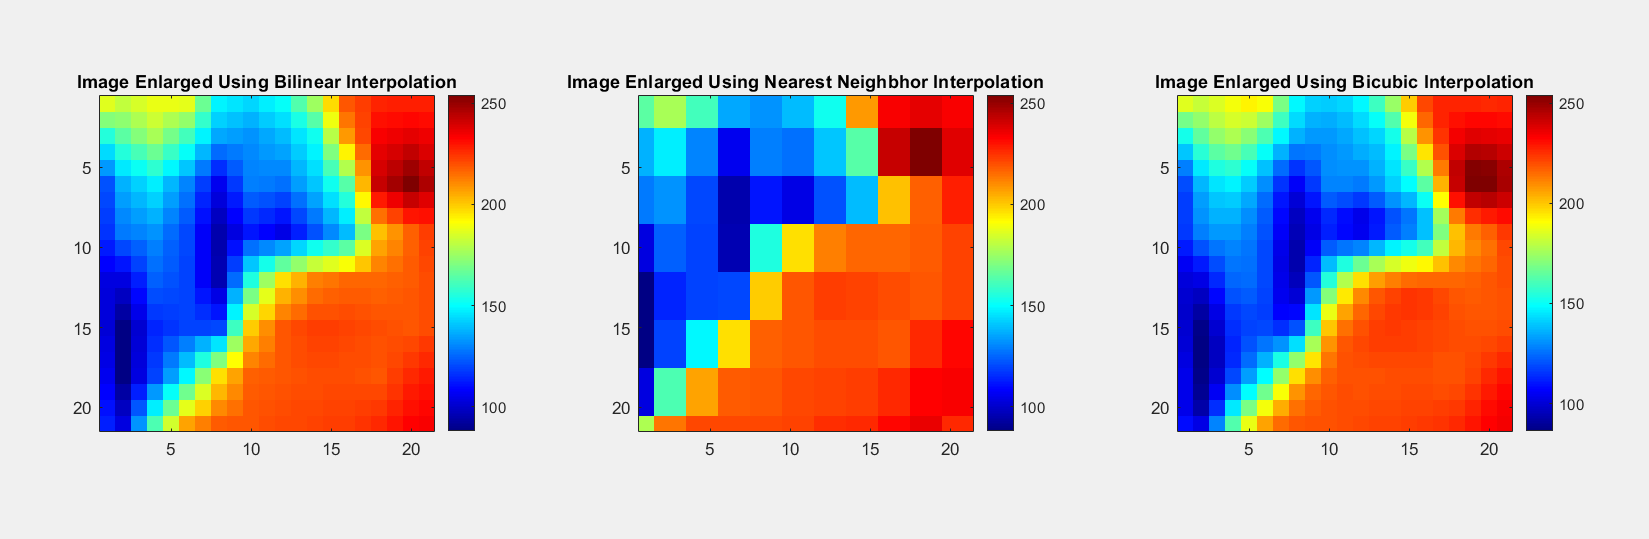
\includegraphics[scale=0.4]{comparision.png}
    \caption{Three interpolation methods}
  \label{fig:6}
\end{figure}

\subsection*{Part F}
Our last task in this question was to rotate the image by $30^{\circ}$ in the clockwise direction. Here we employed the bilinear interpolation method to find function values at the new image grid. Since we generated the image having same size as the original image edges were cut off. Result is shown below.

\begin{figure}[h!]
  \centering
    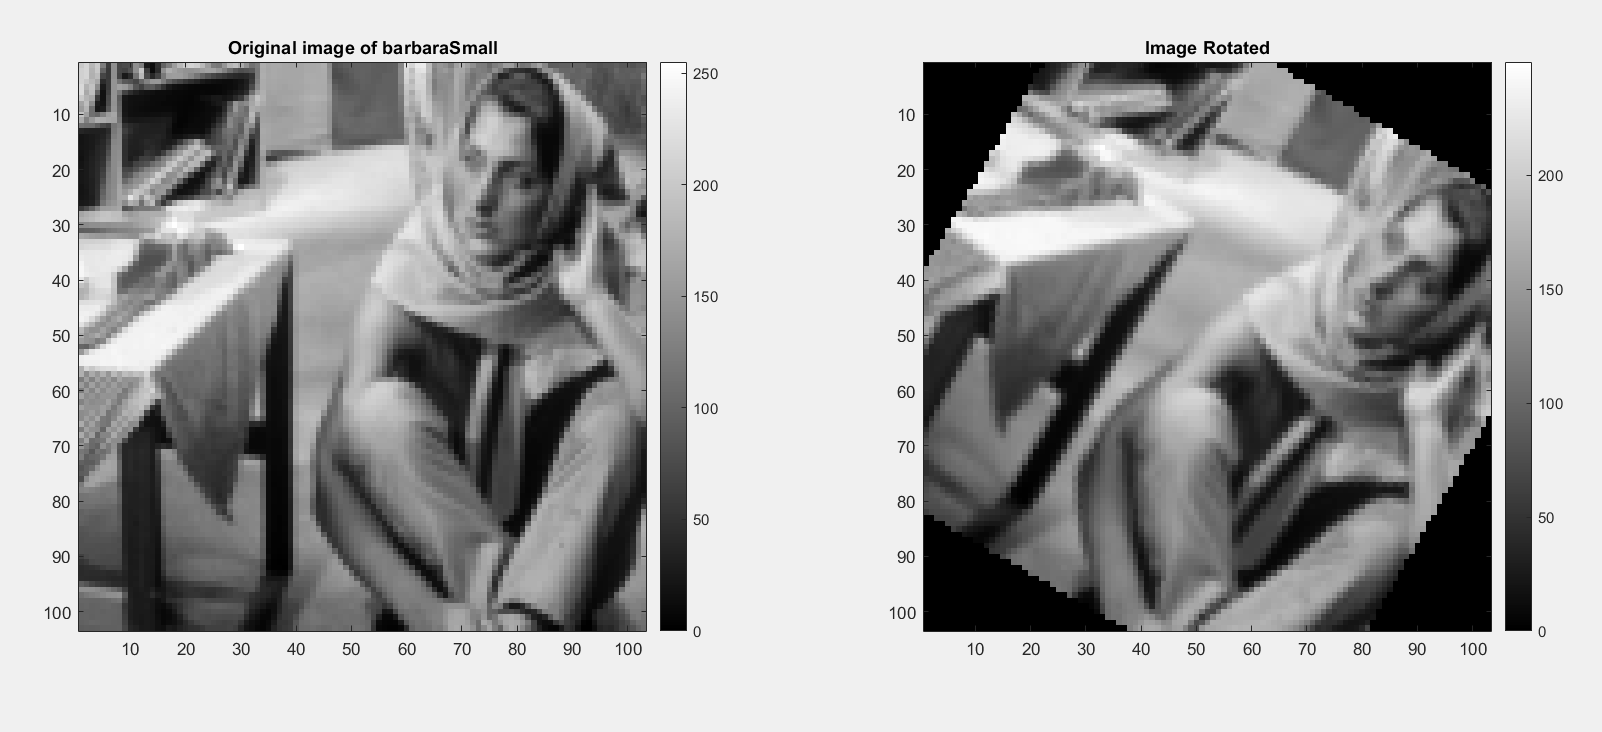
\includegraphics[scale=0.4]{image_rotation.png}
    \caption{Image Rotation by 30^{\circ}}
  \label{fig:7}
\end{figure}

\clearpage

\subsection*{Part G}
The main file myMainScript.m is divided into 6 parts. 
\begin{itemize}
    \item Part A (Image Shrinking)- It contains a simple function, myShrinkImageByFactorD, which just takes the function (image matrix) and shrinking factor d. We shrunk the image size by a factor of d along each dimension using image sub-sampling by sampling / selecting every d-th pixel along the rows and columns. 
    \item Part B (Bilinear Interpolation)- It contains the function myBilinearInterpolation which takes four original image points, a point and area and then calculates the function at the given point using the image points.
    \item Part C (Nearest Neighbor Interpolation)- It contains the function myNearestNeighborInterpolation which takes four original image points, a point and then calculates the image point nearest to the given point and assigns it this value. 
    \item Part D (Bicubic Interpolation)- We first calculate the first derivatives w.r.t. x and y and mixed second derivative for the image grid using difference method. Now we pass these matrices along with the image value, the point at which function value is required and the matrix A\_inv(a constant matrix). It then calculates the value at the given point using the bicubic formula.
    \item Part E (Interpolation Comparison)- It uses the previously defined function to generate a small patch of image to compare the differences in the interpolation techniques.
    \item Part F (Image Rotation)- It contains the function myImageRotation which takes four original image points, a point and then bilinearly interpolates to get the new image grid.
\end{itemize}

\end{document}
